\chapter{Approach}
\label{chap:approach}
In this chapter an overview of the approach used to address the problem of place classification in mobile robotics and concerns regarding implementing novelty detection on it are presented.


\section{Overview}
Graphical models have shown to be useful as they allow to unify the whole set of beliefs that influence a given variable, which is expected to lead to better results than exploiting a single source of information (\autoref{sec:related-work}).

Our approach is based on a \emph{chain graph} representation that combines general purpose knowledge with spatial knowledge and uses probabilistic perception to model variables.

Using a map of the environment or other knowledge (for example given by a user) the graph is built with the variables that the system wants to model (rooms, objects, sensed perceptions).
Connectivity between those variables is then created using default knowledge: such as probabilities of room connectivity or object existence on a given room category.
The low-level sensors are passed through classifiers and their results are plugged into the model.

Using that \emph{graph} the robot can then perform inferences on the variables and estimate the most likely scenario. 
It can be used for example to query about specific variables: that a given room is a kitchen.
Or used to perform high-level reasoning operations such as strategy-planning.


\section{Layers}
The system can be decomposed in four layers:
\emph{Conceptual Layer}, \emph{Categorical Layer}, \emph{Place Layer} and \emph{Sensory Layer}.
Each of them will be presented to the reader in the next sections starting from the high-level \emph{Conceptual Layer} and diving depth into the low-level ones.
\autoref{fig:system-structure} shows the 4 layers and draws lines related to their interaction. A look at the figure with a simultaneous reading of the layers is encouraged.

Special interest for novelty detection and place classification is on the \emph{Conceptual} and \emph{Categorical Layer} as they are the ones responsible for probabilistic modeling and classification.


\subsection{Conceptual Layer}
% TODO graphics:
% World <--> | wall | <--> sensors <--> Graphical model
While the robot moves through the environ it builds a graphical model (\autoref{sec:graphical-models}).
That graph models and relates the unknown variables that the robot tries to extract from reality.
The connections between those random variables can be seen as a filter of possible probability distributions for them \citep{bishop2006pattern}. It is therefore important the way the graph is connected and which variables it models since that is the world model the robot is using.

The description of the modeled variables and factors is given on the next subsections.
\subsubsection*{Modelled Variables}
\begin{description}
\item[Room Category] represents the category the room belongs to. This is the variable used as output to the the place classification.
\item[Room Shape] represents the type of room shape, such as elongated, square. The output of the laser scan is used to condition this variable.
\item[Room Appearance] represents what the room \emph{looks like}, this is associated with the global visual feature classifier.
\item[Object Presence] represents a given object. This variable is conditioned by the object detector which uses local visual features.
\end{description}

\subsubsection*{Modelled Factors}
\begin{description}
\item[Room-Room Connectivity] models the probability that two given rooms are connected. For example class rooms are very likely to be connected to a corridor.
\item[Room-Object Connectivity] models the object presence in a given room.
\item[Observed Room Shape] models the sensed room shape by the classification layer.
\item[Observed Room Appearance] models the sensed room appearance by the classification layer.
\end{description}


\subsection{Categorical Layer}
This layer is responsible from extracting properties from the sensors.
It has classifiers trained to detect several properties from the visual and laser data captured from the robot sensors.

So far the following properties are extracted:
\begin{description}
\item[Object presence] using \emph{local visual features} (\autoref{sec:local-features}).
\item[Place appearance] using \emph{global visual features} (\autoref{sec:global-features}).
\item[Room shape and size] using \emph{geometric features} from 2D laser data to classify properties as: square/elongated and room size.
\item[Landmark detection] uses 2D laser data to detect doors.
\end{description}


\subsection{Place Layer}
The place layer is responsible for the low-level movement and mapping of the environment.
The robot spreads several virtual places markers around the whole environment and maintains connectivity information between them.

By using the door landmarks detected by the categorical layer, it becomes then possible to group the place markers to create the concept of room.

Also this low-level places together with information associating the robot view point with extracted properties allows the system to perform a clever integration over the room properties, avoiding sampling bias, for example coming due to the robot spend too much time in a part of the room (\autoref{sec:accumulation}).

\subsection{Sensory Layer}
This layer captures data from the robots sensors, those include images from cameras, 2D laser scans and odometry from encoders in the movement motors.


\begin{figure}[h]
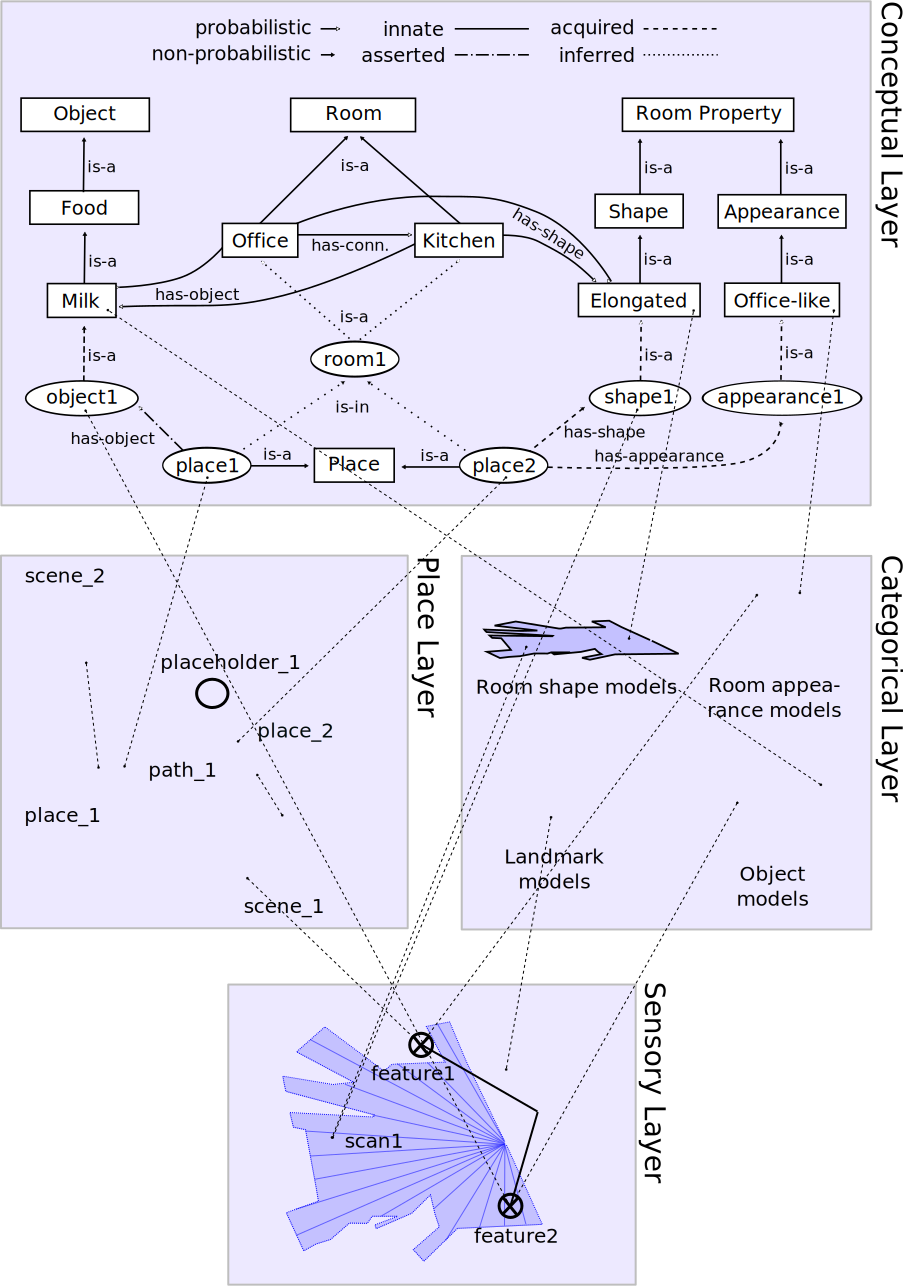
\includegraphics[width=\textwidth]{system-representation/structure}
\caption{In the figure its possible to visualize the interactions of the 4 layers that composed the proposed approach. Novelty detection will have special impact on the \emph{Conceptual} and \emph{Categorical Layers},}
\label{fig:system-structure}
\end{figure}



\section{Novelty Detection}
\label{sec:approach-novelty}
In the previous sections the used approach for the problem of visual place classification was presented.
That system has been used with success by \cite{pronobis2011exploiting} and has demonstrated to be efficient for planning and high-level reasoning under dynamic ambients.

Nonetheless the system has no knowledge about novelty and when presented with a classification task it has to classify the room into one of the room classes it knows.
This poses problems and performance decrease when the robot is deploying into new environments where the room categories or other world variables are novel to the system.

The inability of the robot to handle novel cases (a room which belongs to a category the system was not trained with) is translated at the graphical model not being prepared to handle a unknown variable value.
The detection of novel values (\autoref{sec:novelty-detection}) can be done by triggering on the unconditional probability density for the given input.
Since the presented approach uses a \emph{generative model} we expect such an approach to be feasible.

At a lower-level the system also needs to be extended to handle novelty at the classifiers used to extract properties. In that case novel inputs from the sensors translate as the inability for the classifier to operate correctly and so less confidence must be given to its results. That 
Those classifiers after training do not provide a \emph{generative models} rendering a probabilistic estimation approach infeasible.
For that case other approaches such as \gls{K-PCA} (\autoref{sec:kernel-pca}) will be used to address the problem.

